\chapter{Выбор модели нейронной сети для обучения}

CAPTCHA в формате изображений широко используется для защиты ресурсов от автоматизированных ботов и может быть реализована несколькими способами. Как правило, такие CAPTCHA направлены на проверку способности пользователя распознавать и интерпретировать объекты на изображении. Наиболее распространены два варианта реализации (оба варианта реализации проиллюстрированы на рис.~\ref{fig:example}):

\begin{enumerate}
    \item цельное изображение, содержащее несколько объектов, частично размытых или искажённых, при этом изображение разбито на сетку 3×3 или 4×4. Пользователю предлагается выбрать ячейки, содержащие объекты определённого класса (например, автобусы или светофоры);
    \item составное изображение, сформированное из 9 или 12 отдельных фрагментов (изображений), каждый из которых представляет собой независимое изображение -- зачастую низкого качества, с наложением артефактов или шумов. Задача пользователя -- выбрать те изображения, где присутствует нужный объект.
\end{enumerate}

\begin{figure}[!ht]
    \begin{minipage}[h]{0.49\linewidth}
        \center{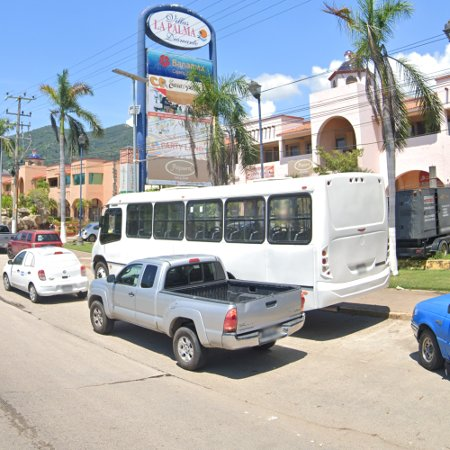
\includegraphics[width=1\linewidth]{imgs/6.jpg} \\ а)}
    \end{minipage}
    \hfill
    \begin{minipage}[h]{0.49\linewidth}
        \center{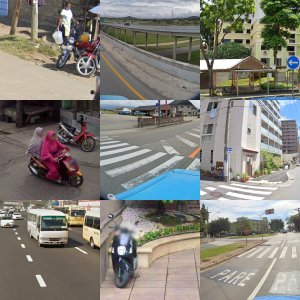
\includegraphics[width=1\linewidth]{imgs/8.jpg} \\ б)}
    \end{minipage}
    \caption{\centering Изображения CAPTCHA с размером сетки 3×3: а) -- цельное, б) -- составное.}
    \label{fig:example}
\end{figure}
\vspace{-0.5cm}

Такие CAPTCHA требуют от системы автоматического анализа способности как к глобальному восприятию изображения, так и к локальной интерпретации его фрагментов. Соответственно, модель, предназначенная для решения данной задачи, должна поддерживать:

\begin{enumerate}
    \item классификацию объектов на уровне отдельных изображений (для CAPTCHA, основанных на отдельных картинках в сетке);
    \item локализацию и сегментацию объектов с высокой точностью, чтобы корректно определить границы объектов в пределах ячеек, особенно в случаях, когда объект может частично заходить за границу между ячейками.
\end{enumerate}

Для решения этих задач были рассмотрены следующие современные архитектуры нейронных сетей:

\begin{enumerate}
    \item YOLO (You Only Look Once) -- однопроходная модель, объединяющая классификацию и регрессию ограничивающих рамок в одной свёрточной архитектуре. Отличается высокой скоростью и хорошей точностью~\cite{redmon2016yolov2, UltralyticsYOLODocs};
    \item Faster R-CNN -- двухступенчатая модель, в которой сначала генерируются области предложений, а затем выполняется классификация и уточнение рамок. Обладает высокой точностью, но уступает в скорости~\cite{ren2015fasterrcnn};
    \item DETR (DEtection TRansformer) -- основана на архитектуре трансформеров, что позволяет эффективно моделировать глобальные взаимосвязи между объектами. Подходит для задач с большим количеством контекстных зависимостей, но требует больше ресурсов для обучения~\cite{carion2020detr}.
\end{enumerate}

Среди этих архитектур было принято решение использовать YOLOv8 по следующим причинам~\cite{UltralyticsYOLOv8}:

\begin{enumerate}
    \item высокая производительность: YOLOv8 показывает высокую скорость обработки изображений без значительного ущерба для точности, что критично в условиях, когда необходимо обрабатывать CAPTCHA в реальном времени;
    \item гибкость и масштабируемость: модель предоставляет множество предобученных вариантов с различной глубиной и числом параметров (версии n, s, m, l, x), что позволяет использовать как на слабых, так и на производительных устройствах;
    \item широкая поддержка и документация: YOLOv8 имеет активное сообщество, подробную документацию и регулярно обновляется, что значительно упрощает интеграцию и адаптацию модели под пользовательские задачи;
    \item поддержка сегментации: в отличие от более ранних версий, YOLOv8 поддерживает не только детекцию, но и сегментацию объектов, что особенно важно для задач, где необходимо точно определить область объекта внутри изображения;
    \item дообучение на пользовательских данных: YOLOv8 позволяет эффективно дообучать модель на собственных датасетах, что особенно важно при работе с CAPTCHA-изображениями, содержащими специфические классы объектов и нестандартные искажения.
\end{enumerate}

Кроме того, модель YOLOv8 была успешно протестирована в задачах, близких по структуре к CAPTCHA: детекции дорожных знаков, транспортных средств, пешеходов и других объектов в сложных условиях съёмки, что подтверждает её универсальность и применимость к рассматриваемой задаче.

Таким образом, YOLOv8 является наиболее сбалансированным выбором, обеспечивающим как точную классификацию, так и локализацию объектов в условиях ограниченных ресурсов и с возможностью адаптации под специфику визуальных CAPTCHA.
